\documentclass[10pt]{article}
\usepackage[margin=0.72in]{geometry}
\usepackage{booktabs}
\usepackage{graphicx}
\usepackage{caption}
\usepackage{microtype}
\usepackage{hyperref}
\usepackage{xcolor}
\usepackage{longtable}
\captionsetup{font=small,labelfont=bf}
\graphicspath{{figures/}}
\setlength{\parskip}{0.45em}
\setlength{\parindent}{0pt}

\title{Preliminary Dense-RHS CoRL Compact Results}
\author{Autogenerated from local TD-MPC2-JAX run artifacts}
\date{}

\begin{document}
\maketitle

\textbf{Scope.} This preliminary report summarizes the completed compact campaign ``dense\_rhs\_corl\_compact\_v2'' using local metric caches refreshed from the NCC run directories. It is intended as an internal CoRL-style evidence package, not as the final v3 matrix. The following environment is excluded from all results and plots: fish-swim.

\textbf{Headline.} Across 30 matched valid seed pairs, Adaptive RHS changes final score by \textbf{5.90\% $\pm$ 24.00\%} relative to the fixed TD-MPC2 paper horizon, with an RHS win rate of \textbf{70.00\%}. The summary excludes 0 missing, nonfinite, or unmatched pairs.

\section*{Experimental Setup}
We compare the TD-MPC2 fixed paper horizon against Adaptive RHS under matched environment, regime, and seed cells. Environments are quadruped-run, cheetah-run, hopper-hop, finger-turn\_hard, cartpole-swingup; regimes are clean and chaos; seeds are 1, 7, 15; training budget is 500000 environment steps. All rows come from \texttt{experiments/corl\_compact\_v2\_ledger.csv}; each row records the SLURM job id, git commit, remote run directory, score, runtime, and checkpoint status.

\section*{Aggregate Result}
\begin{center}
\begin{tabular}{lllll}
\toprule
Scope & n & RHS delta (\%) & RHS wins & Runtime ratio \\
\midrule
all valid pairs & 30 & 5.90 $\pm$ 24.00 & 70.00\% & 1.13 \\
chaos & 15 & 11.43 $\pm$ 31.37 & 73.33\% & 1.13 \\
clean & 15 & 0.37 $\pm$ 11.99 & 66.67\% & 1.13 \\
\bottomrule
\end{tabular}

\end{center}

\section*{Full Matched Results}
\begingroup
\scriptsize
\setlength{\tabcolsep}{3.2pt}
\begin{longtable}{lllrrrrr}
\toprule
Environment & Regime & Seed & Fixed & RHS & $\Delta$ (\%) & Fixed h & RHS h \\
\midrule
\endfirsthead
\toprule
Environment & Regime & Seed & Fixed & RHS & $\Delta$ (\%) & Fixed h & RHS h \\
\midrule
\endhead
cartpole-swingup & chaos & 1 & 814.1 & 816.4 & +0.28 & 1.76 & 2.04 \\
cartpole-swingup & chaos & 7 & 856.5 & 861.5 & +0.59 & 1.78 & 2.15 \\
cartpole-swingup & chaos & 15 & 859.2 & 860.6 & +0.16 & 1.81 & 2.18 \\
cartpole-swingup & clean & 1 & 882.1 & 864.9 & -1.95 & 1.38 & 1.95 \\
cartpole-swingup & clean & 7 & 878.4 & 882.4 & +0.45 & 1.37 & 1.62 \\
cartpole-swingup & clean & 15 & 864.5 & 879.8 & +1.77 & 1.37 & 1.86 \\
cheetah-run & chaos & 1 & 354.5 & 501.1 & +41.35 & 1.94 & 2.36 \\
cheetah-run & chaos & 7 & 515.4 & 595.9 & +15.64 & 1.94 & 2.10 \\
cheetah-run & chaos & 15 & 528.2 & 540.9 & +2.41 & 1.95 & 2.19 \\
cheetah-run & clean & 1 & 926.2 & 946.6 & +2.20 & 1.51 & 1.62 \\
cheetah-run & clean & 7 & 944.0 & 942.7 & -0.14 & 1.50 & 1.64 \\
cheetah-run & clean & 15 & 850.7 & 905.6 & +6.45 & 1.50 & 1.63 \\
finger-turn-hard & chaos & 1 & 651.0 & 448.7 & -31.08 & 1.95 & 2.05 \\
finger-turn-hard & chaos & 7 & 580.5 & 838.8 & +44.50 & 1.94 & 2.21 \\
finger-turn-hard & chaos & 15 & 510.1 & 753.5 & +47.71 & 1.97 & 2.06 \\
finger-turn-hard & clean & 1 & 772.7 & 918.8 & +18.91 & 1.49 & 1.66 \\
finger-turn-hard & clean & 7 & 818.2 & 917.0 & +12.07 & 1.50 & 1.60 \\
finger-turn-hard & clean & 15 & 884.6 & 928.9 & +5.01 & 1.50 & 1.60 \\
hopper-hop & chaos & 1 & 166.8 & 278.1 & +66.71 & 2.15 & 2.46 \\
hopper-hop & chaos & 7 & 292.4 & 159.1 & -45.59 & 2.14 & 2.58 \\
hopper-hop & chaos & 15 & 158.2 & 139.0 & -12.17 & 2.17 & 2.55 \\
hopper-hop & clean & 1 & 542.8 & 570.1 & +5.04 & 1.72 & 1.83 \\
hopper-hop & clean & 7 & 514.9 & 469.7 & -8.78 & 1.71 & 1.86 \\
hopper-hop & clean & 15 & 559.3 & 357.9 & -36.00 & 1.73 & 1.87 \\
quadruped-run & chaos & 1 & 660.8 & 732.9 & +10.90 & 2.43 & 2.64 \\
quadruped-run & chaos & 7 & 807.8 & 722.1 & -10.60 & 2.41 & 2.56 \\
quadruped-run & chaos & 15 & 576.1 & 810.0 & +40.59 & 2.42 & 2.56 \\
quadruped-run & clean & 1 & 881.8 & 913.6 & +3.60 & 1.93 & 2.13 \\
quadruped-run & clean & 7 & 879.3 & 839.9 & -4.48 & 1.96 & 2.10 \\
quadruped-run & clean & 15 & 911.0 & 923.8 & +1.41 & 1.99 & 2.25 \\
\bottomrule
\end{longtable}
\endgroup


\section*{Learning Curves}
\begin{figure}[h]
  \centering
  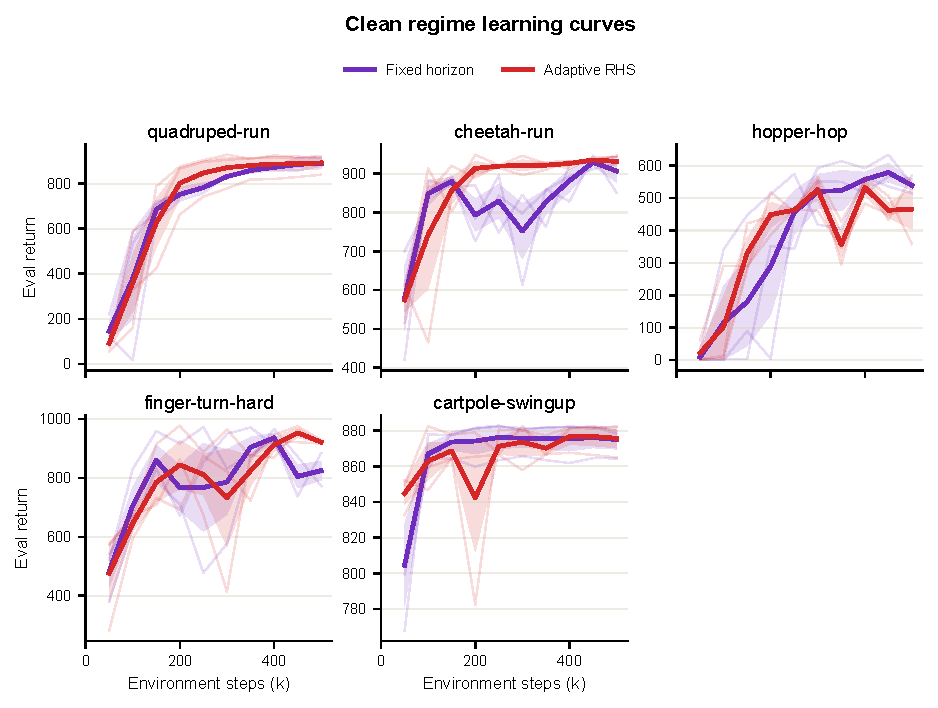
\includegraphics[width=\linewidth]{fig_learning_curves_clean.pdf}
  \caption{Clean-regime evaluation return. Thin traces are individual seeds; bold traces show the seed mean with standard error.}
\end{figure}

\begin{figure}[h]
  \centering
  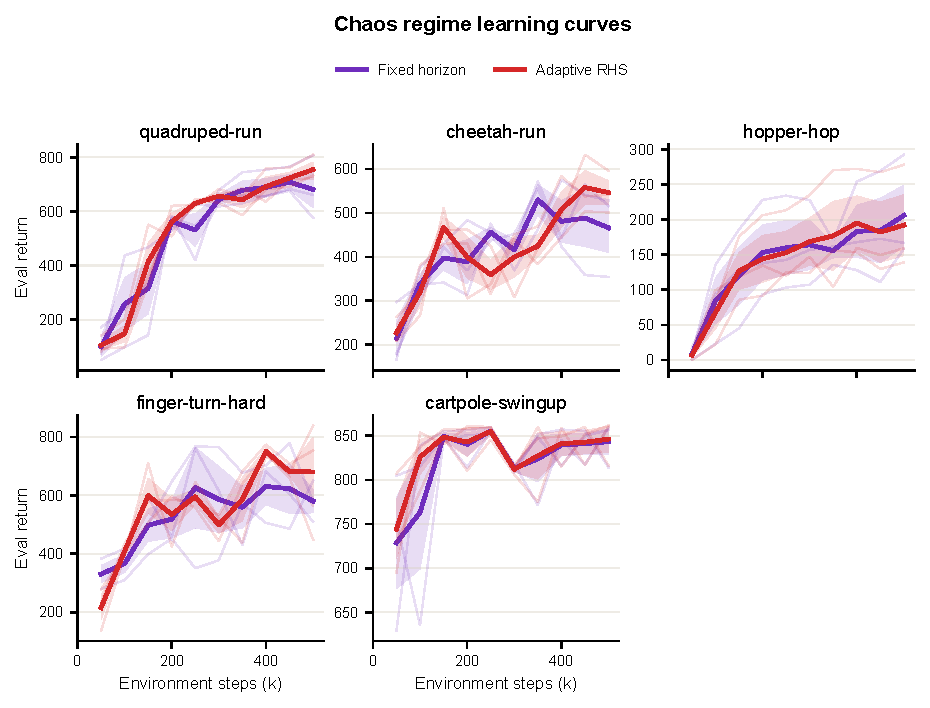
\includegraphics[width=\linewidth]{fig_learning_curves_chaos.pdf}
  \caption{Chaos-regime evaluation return under matched randomized/noisy evaluation.}
\end{figure}

\clearpage
\section*{Matched Percent Delta}
\begin{figure}[h]
  \centering
  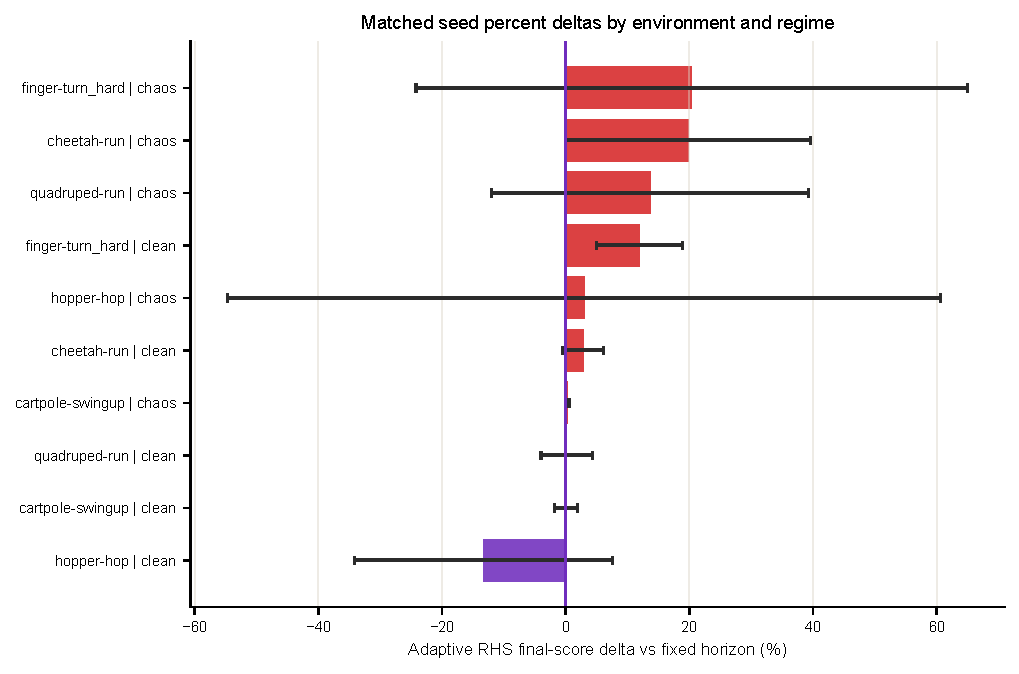
\includegraphics[width=0.92\linewidth]{fig_percent_delta_summary.pdf}
  \caption{Per-environment and per-regime Adaptive RHS percent delta against the matched fixed-horizon baseline. Error bars are across seeds.}
\end{figure}

\begin{center}
\begin{tabular}{llllll}
\toprule
Environment & Regime & n & RHS delta (\%) & RHS wins & RHS h \\
\midrule
cartpole-swingup & chaos & 3 & 0.34 $\pm$ 0.22 & 100.0\% & 2.12 \\
cartpole-swingup & clean & 3 & 0.09 $\pm$ 1.89 & 66.67\% & 1.81 \\
cheetah-run & chaos & 3 & 19.80 $\pm$ 19.80 & 100.0\% & 2.22 \\
cheetah-run & clean & 3 & 2.84 $\pm$ 3.34 & 66.67\% & 1.63 \\
finger-turn\_hard & chaos & 3 & 20.38 $\pm$ 44.59 & 66.67\% & 2.11 \\
finger-turn\_hard & clean & 3 & 11.99 $\pm$ 6.95 & 100.0\% & 1.62 \\
hopper-hop & chaos & 3 & 2.98 $\pm$ 57.66 & 33.33\% & 2.53 \\
hopper-hop & clean & 3 & -13.25 $\pm$ 20.88 & 33.33\% & 1.85 \\
quadruped-run & chaos & 3 & 13.63 $\pm$ 25.71 & 66.67\% & 2.59 \\
quadruped-run & clean & 3 & 0.18 $\pm$ 4.18 & 66.67\% & 2.16 \\
\bottomrule
\end{tabular}

\end{center}

\section*{Efficiency and Pareto View}
\begin{figure}[h]
  \centering
  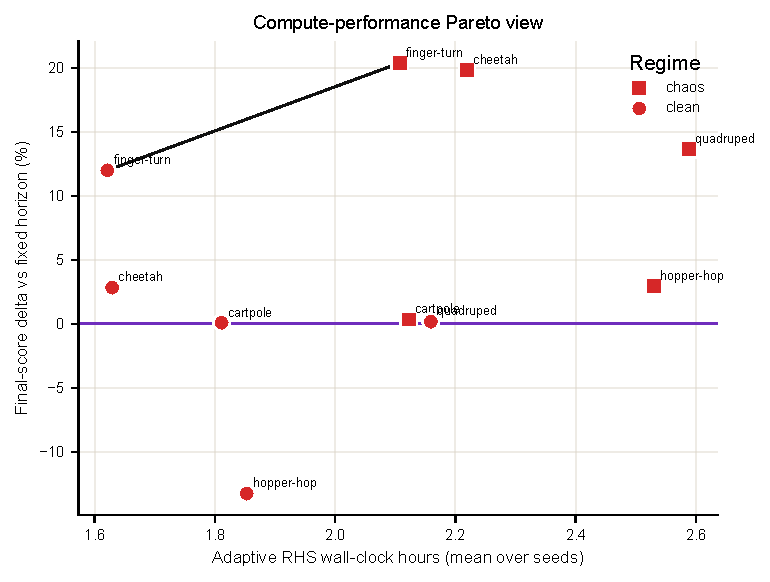
\includegraphics[width=0.72\linewidth]{fig_pareto_frontier.pdf}
  \caption{Compute-performance Pareto view. The x-axis is mean Adaptive RHS wall-clock hours and the y-axis is normalized final-score delta versus the matched fixed-horizon baseline; the black line highlights nondominated points.}
\end{figure}

\begin{figure}[h]
  \centering
  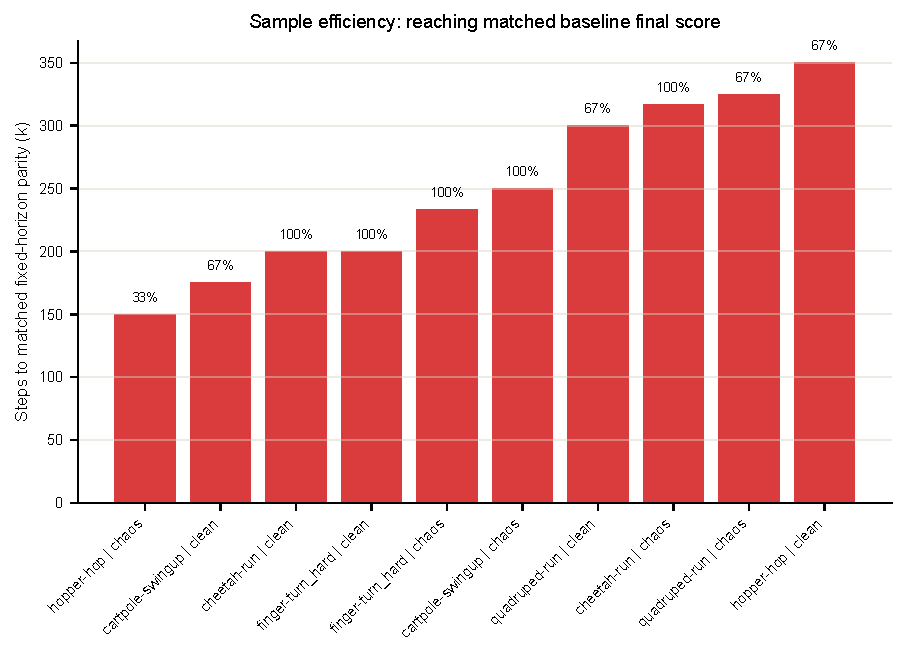
\includegraphics[width=0.86\linewidth]{fig_time_to_parity.pdf}
  \caption{Sample efficiency, measured as the first Adaptive RHS evaluation point that reaches the matched fixed-horizon final score. Labels above bars indicate the fraction of seeds reaching parity.}
\end{figure}

\clearpage
\section*{RHS Diagnostics}
\begin{figure}[h]
  \centering
  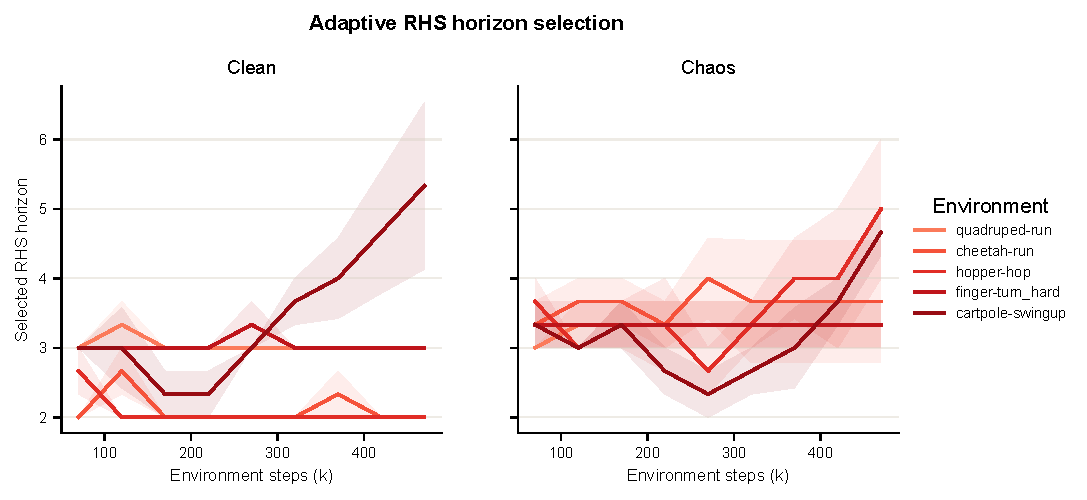
\includegraphics[width=\linewidth]{fig_horizon_diagnostics.pdf}
  \caption{Adaptive RHS selected horizon over training, averaged across seeds.}
\end{figure}

\begin{figure}[h]
  \centering
  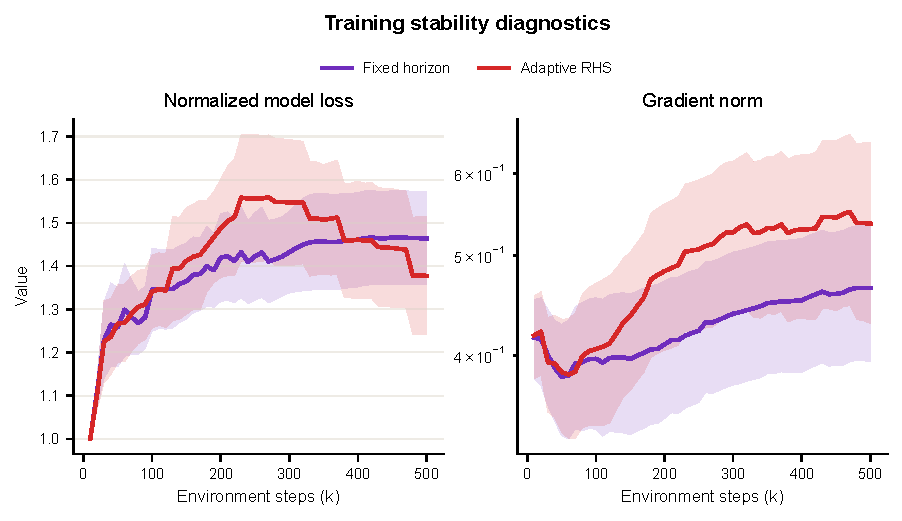
\includegraphics[width=0.88\linewidth]{fig_loss_diagnostics.pdf}
  \caption{Training stability diagnostics pooled across runs. Total loss is normalized per run by its first finite value; gradient norms use a log axis.}
\end{figure}

\section*{Limitations}
This is a preliminary report for the completed compact run after applying the report-level environment filter (60 retained terminal rows). Fish-swim is intentionally omitted because it was later removed from the v3 final matrix after isolated MJX chaos-push diagnostics exposed nonfinite state/reward failures. The final v3 package should reuse the same report template with the updated environment set and six seeds.

\end{document}
